\documentclass[aspectratio=169]{beamer}
\usepackage[utf8]{inputenc}
\usepackage[T1]{fontenc}
\graphicspath{{images/}} % path containing image files

% required fields
\title{There Is No Largest Prime Number}
\author[Euclid]{Euclid of Alexandria}
\date[\today]{27th International Symposium of Prime Numbers - \today} % date and/or event
% optional fields; comment if not used
\subtitle{The proof uses \textit{reductio ad absurdum}.}
\institute[UofA]{University of Alexandria}
% additional metadata; leave empty {} if not applicable and edit/remove backmatter slides w/ copyright info appropriately
\def \keywords {numbers, beamer, latex}
\def \copyrightinfo {Copyright \textcopyright~\the\year{} Euclid of Alexandria, licensed under the CC-BY 4.0 license (unless otherwise stated).}
\def \licenseurl {https://creativecommons.org/licenses/by/4.0/}

\usetheme{uis}
\addbibresource{sample.bib} % sample bibliography

\begin{document}

\begin{frame}
  \titlepage
\end{frame}

\begin{frame}{Table of Contents}
  \tableofcontents 
  % sections and subsections will be printed in the toc
\end{frame}
  
\section{First Section} % -----------------------------------------
  
\subsection{Subsection Example} % ----------------------------------
  
\begin{frame}{Table of Contents} 
  \tableofcontents[currentsection] % highlight current section in the toc
\end{frame}
  
\begin{frame}{Bullet Points}
  \begin{itemize}
    \item Lorem ipsum dolor sit amet, consectetur adipiscing elit
    \item Aliquam blandit faucibus nisi, sit amet dapibus enim tempus eu
    \item Nulla commodo, erat quis gravida posuere, elit lacus lobortis est, quis porttitor odio mauris at libero
    \item Nam cursus est eget velit posuere pellentesque
    \item Vestibulum faucibus velit a augue condimentum quis convallis nulla gravida
  \end{itemize}
\end{frame}

\begin{frame}[allowframebreaks]{Paragraphs of Text with Automatic Frame Breaks} % Untitled frame
  Sed iaculis dapibus gravida. Morbi sed tortor erat, nec interdum arcu. Sed id lorem lectus. Quisque viverra augue id sem ornare non aliquam nibh tristique. Aenean in ligula nisl. Nulla sed tellus ipsum. Donec vestibulum ligula non lorem vulputate fermentum accumsan neque mollis.\\~\\
  Sed diam enim, sagittis nec condimentum sit amet, ullamcorper sit amet libero. Aliquam vel dui orci, a porta odio. Nullam id suscipit ipsum. Aenean lobortis commodo sem, ut commodo leo gravida vitae. Pellentesque vehicula ante iaculis arcu pretium rutrum eget sit amet purus. Integer ornare nulla quis neque ultrices lobortis. Vestibulum ultrices tincidunt libero, quis commodo erat ullamcorper id. \\~\\
  Lorem ipsum dolor sit amet, consectetur adipiscing elit. Integer lectus nisl, ultricies in feugiat rutrum, porttitor sit amet augue. Aliquam ut tortor mauris. Sed volutpat ante purus, quis accumsan dolor.\\~\\
  Pellentesque sed tellus purus. Class aptent taciti sociosqu ad litora torquent per conubia nostra, per inceptos himenaeos. Vestibulum quis magna at risus dictum tempor eu vitae velit. Suspendisse tincidunt sagittis gravida. Curabitur condimentum, enim sed venenatis rutrum, ipsum neque consectetur orci, sed blandit justo nisi ac lacus.
\end{frame}  

\begin{frame}{Blocks of Highlighted Text}
  \begin{block}{Block 1}
    Lorem ipsum dolor sit amet, consectetur adipiscing elit. Integer lectus nisl, ultricies in feugiat rutrum, porttitor sit amet augue. Aliquam ut tortor mauris. Sed volutpat ante purus, quis accumsan dolor.
  \end{block}
  \begin{block}{Block 2}
    Pellentesque sed tellus purus. Class aptent taciti sociosqu ad litora torquent per conubia nostra, per inceptos himenaeos. Vestibulum quis magna at risus dictum tempor eu vitae velit.
  \end{block}
\end{frame}
  
\begin{frame}{Multiple Columns}
  \begin{columns}[c] % The "c" option specifies centred vertical alignment while the "t" option is used for top vertical alignment
    \column{.45\textwidth} % Left column and width
    \textbf{Heading}
    \begin{enumerate}
      \item Statement
      \item Explanation
      \item Example
    \end{enumerate}
    \column{.45\textwidth} % Right column and width
    Lorem ipsum dolor sit amet, consectetur adipiscing elit. Integer lectus nisl, ultricies in feugiat rutrum, porttitor sit amet augue. Aliquam ut tortor mauris. Sed volutpat ante purus, quis accumsan dolor.
  \end{columns}
\end{frame}

\section{Second Section} % ---------------------------------------
  
\begin{frame}{Table of Contents} 
  \tableofcontents[currentsection] 
\end{frame}
  
\begin{frame}{Table}
  \begin{table}
    \setbeamertemplate{caption}{\insertcaption} % if label is not required
    \caption{Table caption}
    \begin{tabular}{l l l}
      \toprule
      \textbf{Treatments} & \textbf{Response 1} & \textbf{Response 2}\\
      \midrule
      Treatment 1 & 0.0003262 & 0.562 \\
      Treatment 2 & 0.0015681 & 0.910 \\
      Treatment 3 & 0.0009271 & 0.296 \\
      \bottomrule
    \end{tabular}
  \end{table}
\end{frame}
  
\begin{frame}{Theorem}
  \begin{theorem}[Mass--energy equivalence]
    $E = mc^2$
  \end{theorem}
  \begin{theorem}[Another example equation]
    $S_n = \frac{X_1 + X_2 + \cdots + X_n}{n} = \frac{1}{n}\sum_{i}^{n} X_i$
  \end{theorem}
\end{frame}

\begin{frame}[fragile]{Verbatim} % Need to use the fragile option when verbatim is used in the slide
  \begin{example}[Theorem Slide Code]
    \begin{verbatim}
    \begin{frame}
    \frametitle{Theorem}
    \begin{theorem}[Mass--energy equivalence]
    $E = mc^2$
    \end{theorem}
    \end{frame}\end{verbatim}
  \end{example}
\end{frame}

\begin{frame}{Figure}
  \begin{figure}
    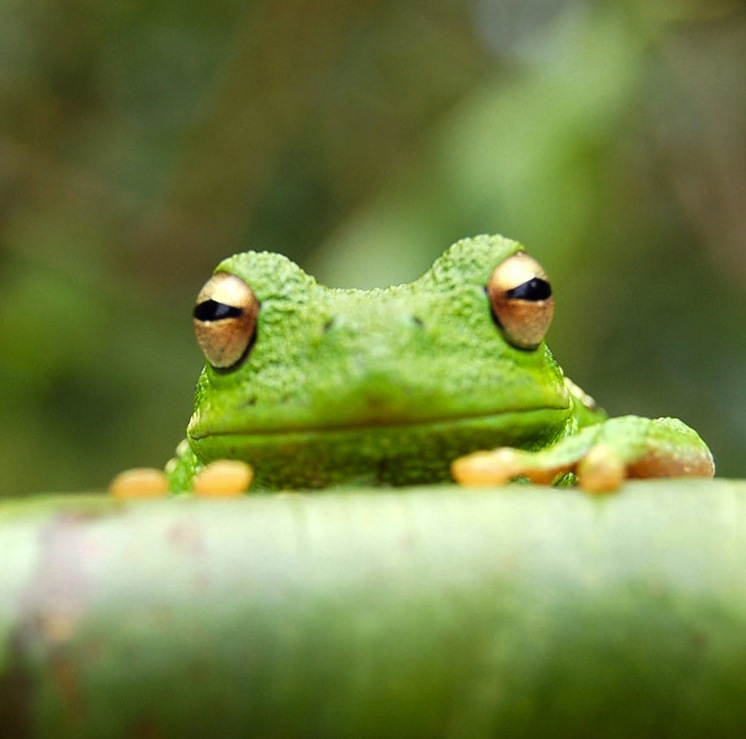
\includegraphics[width=.2\linewidth]{frog}
    \setbeamertemplate{caption}{\insertcaption} % if label is not required
    \caption{Figure caption}
  \end{figure}
\end{frame}

\begin{frame}[fragile]{Citation} % Need to use the fragile option when verbatim is used in the slide
  An example of the \verb|\cite| command to cite within the presentation:\\~\\
  This statement requires a citation \cite{westfahl:space}. This statement requires three citations \cite{angenendt,knuth:ct:b,aristotle:rhetoric}. This statement requires multiple citations \cite{angenendt,knuth:ct:b,aristotle:rhetoric,westfahl:space}.
\end{frame}

\begin{frame} % thank you slide
  \Huge\centering{Thank you for your attention!}\large\\~\\
  \href{mailto:euclid@alexandria.edu}{\ttfamily euclid@alexandria.edu} % email and other contact info can go here
\end{frame}

% backmatter --------------------------------
\appendix 
\begin{frame}[allowframebreaks]{References}
% if you would like a citation which is not used in the main body to be displayed in the references, use the \nocite{bibid} command
  \nocite{vangennep:related,ctan,aksin,bertram,doody,sigfridsson,spiegelberg,springer,aristotle:poetics,britannica}
  \printbibliography
\end{frame}

\section{Copyright info}
\begin{frame} % copyright info
  \copyrightinfo\\~\\
  \url{\licenseurl}\\~\\
\end{frame}

\end{document}
